\usetikzlibrary {automata,positioning}
% "A|B"
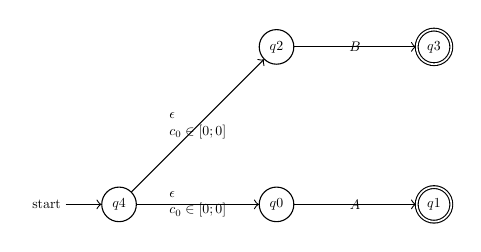
\begin{tikzpicture}[every node/.style={scale=0.5}]
    \node[state] at (2, 0)(q0){$q0$};
    \node[state, accepting] at (4, 0)(q1){$q1$};
    \node[state] at (2, 2)(q2){$q2$};
    \node[state, accepting] at (4, 2)(q3){$q3$};
    \node[state, initial] at (0, 0)(q4){$q4$};
    
    \path[->]
        (q0)edge node[align=left]{$A$}(q1)
        (q2)edge node[align=left]{$B$}(q3)
        (q4)edge node[align=left]{$\epsilon$\\$c_0\in[0;0]$}(q0)
        (q4)edge node[align=left]{$\epsilon$\\$c_0\in[0;0]$}(q2)
        ;
\end{tikzpicture}